\subsubsection{Conceptos}\label{sec:0z0z2Conceptos}

\paragraph{Oscilador}
Un oscilador se compone de un elemento resonante y un elemento amplificador conectados en feedback (ver figura \ref{fig:basicOscilator}) que lo que hace es amplificar el componente resonante mientras los otros componentes frecuenciales se eliminan. Para que este esquema logre oscilar en la frecuencia deseada comenzando con la amplificación del ruido blanco, se necesita una amplificación de loop igual o mayor a 1 y un desfase total de 360 grados (en fase). Nótese que la alternativa de alimentar el oscilador con la frecuencia de interés no tiene sentido porque significaría necesariamente construir un oscilador previamente.

\begin{figure}[H]
    \centering
    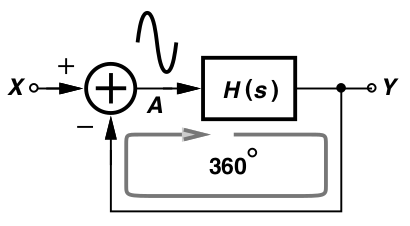
\includegraphics[width=6cm]{Images/1.png}
    \caption{Esquema básico de un oscilador. Sacado de \cite{razavi}}
    \label{fig:basicOscilator}
\end{figure}

Para la sección de amplificación, usar un amplificador operacional no es posible en muchos casos porque el comportamiento de amplificación se pierde en frecuencias altas, por lo que es recomendable usar BJT's o MOSFET. 


\paragraph{BJT}
En cuanto al transistor BJT, varias características son importantes para construir exitosamente el amplificador. Entre ellas:
\begin{itemize}
    \item Resistencias equivalentes. En las compuertas (útil para el acople de impedancias). Ver figura \ref{fig:ReqBJT}
    \item Relación de amplificación de Emisor común. 
    \item Valores específicos. 
\end{itemize}
Se sabe entonces que, por ejemplo, la resistencia de colector equivalente es: 
\begin{align}
    V_C=
\end{align}

\begin{figure}[H]
    \centering
    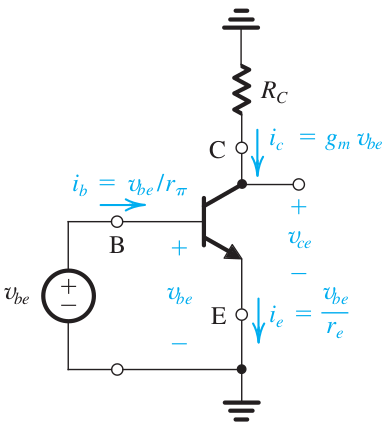
\includegraphics[width=5cm]{Images/11.png}
    \caption{Resistencias equivalentes de un BJT NPN. Sacado de \cite{sedra}}
    \label{fig:ReqBJT}
\end{figure}

\paragraph{Amplificador de emisor común}


El amplificador de emisor común invierte la fase 180 grados y una ganancia dada por la expresión \ref{eq:GainCommonEmisor}. 
\begin{equation}
    \label{eq:GainCommonEmisor}
    -gm\frac{R_C}{1+gmR_E} = \frac{R_C}{R_E+\frac{1}{gm}} \approx \xrightarrow{R_E>>\frac1{gm}} \approx \frac{R_C}{R_E}
\end{equation}
En la figura \ref{fig:GeneralCommonEmitter} se muestra de forma general la idea de esta configuración. Con la salida en el colector, la entrada en la base y el emisor a tierra. 

\begin{figure}[H]
    \centering
    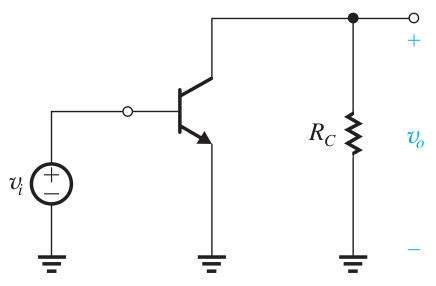
\includegraphics[width=4cm]{Images/12.png}
    \caption{Esquema general de emisor común}
    \label{fig:GeneralCommonEmitter}
\end{figure}

\paragraph{Oscilador Colpitts}
El oscilador Colpitts (ver figura \ref{fig:0z0z2:1}) utiliza un circuito tanque de dos capacitores y un inductor que resuenan en la frecuencia de diseño. La amplificación de esta sección está dada por la relación de los capacitores mientras que la relación entre los tres elementos describe la frecuencia de resonancia: 

\begin{align}
    \label{eq:2}
    A &= -\frac{C_1}{C_2} \\    
    \omega &= 2\pi f = \sqrt{\frac{C_1+C_2}{C_1C_2L}} \\
\end{align} Ecuaciones obtenidas de \cite{notasCurso} y \cite{aaron_danner_colpitts_2023}

\begin{figure}[H]
    \begin{subfigure}{0.3\textwidth}
        \centering
        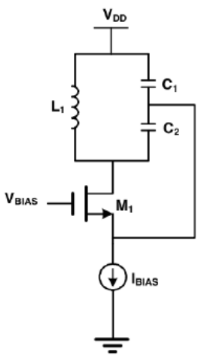
\includegraphics[height=6cm]{Images/2.png} 
            \caption{Colpitts con MOSFET}
    \end{subfigure}
    \begin{subfigure}{0.7\textwidth}
       \centering
        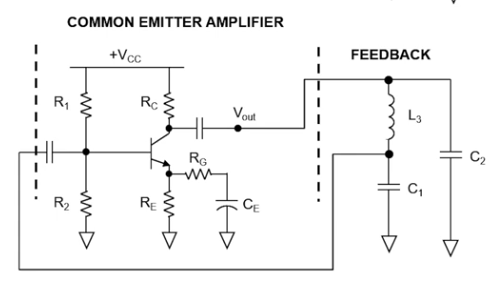
\includegraphics[height=6cm]{Images/3.png}
        \caption{Colpitts con BJT NPN}
    \end{subfigure}
    \caption{Comparación de dos esquemas de osciladores Colpitts que usan un transistor como etapa de amplificación.}
    \label{fig:0z0z2:1}
\end{figure}

\paragraph{Polarización}

Es interesante notar como en las dos imágenes en la figura \ref{fig:0z0z2:1} se tienen aparentemente dos esquemas distintos. Sin embargo, la idea principal se mantiene y entre los cambios principales se encuentran el tipo de transistor y la forma en la que se polariza el transistor. (fuente de corriente y fuente de tensión).

La polarización por fuente de corriente se usa principalmente en circuitos donde se requiere una corriente constante, como en los circuitos de referencia de corriente. Entre las ventajas de utilizar fuentes de corriente se tienen:
\begin{itemize}
    \item Estabilidad de Corriente: La corriente a través del transistor se mantiene constante, lo cual es útil para aplicaciones que requieren una corriente fija independientemente de las variaciones en la tensión de alimentación o en el transistor.
    \item Precisión: La fuente de corriente proporciona una polarización muy precisa, que es crucial en aplicaciones analógicas de alta precisión.
\end{itemize}

Entre las desventajas de utilizar fuentes de corriente se tienen:

\begin{itemize}
    \item Costos y Disponibilidad: Las fuentes de corriente son menos comunes y pueden ser más costosas que las fuentes de tensión.
\end{itemize}

